\documentclass[serif]{beamer}\usepackage[]{graphicx}\usepackage[]{color}
%% maxwidth is the original width if it is less than linewidth
%% otherwise use linewidth (to make sure the graphics do not exceed the margin)
\makeatletter
\def\maxwidth{ %
  \ifdim\Gin@nat@width>\linewidth
    \linewidth
  \else
    \Gin@nat@width
  \fi
}
\makeatother

\definecolor{fgcolor}{rgb}{0.345, 0.345, 0.345}
\newcommand{\hlnum}[1]{\textcolor[rgb]{0.686,0.059,0.569}{#1}}%
\newcommand{\hlstr}[1]{\textcolor[rgb]{0.192,0.494,0.8}{#1}}%
\newcommand{\hlcom}[1]{\textcolor[rgb]{0.678,0.584,0.686}{\textit{#1}}}%
\newcommand{\hlopt}[1]{\textcolor[rgb]{0,0,0}{#1}}%
\newcommand{\hlstd}[1]{\textcolor[rgb]{0.345,0.345,0.345}{#1}}%
\newcommand{\hlkwa}[1]{\textcolor[rgb]{0.161,0.373,0.58}{\textbf{#1}}}%
\newcommand{\hlkwb}[1]{\textcolor[rgb]{0.69,0.353,0.396}{#1}}%
\newcommand{\hlkwc}[1]{\textcolor[rgb]{0.333,0.667,0.333}{#1}}%
\newcommand{\hlkwd}[1]{\textcolor[rgb]{0.737,0.353,0.396}{\textbf{#1}}}%
\let\hlipl\hlkwb

\usepackage{framed}
\makeatletter
\newenvironment{kframe}{%
 \def\at@end@of@kframe{}%
 \ifinner\ifhmode%
  \def\at@end@of@kframe{\end{minipage}}%
  \begin{minipage}{\columnwidth}%
 \fi\fi%
 \def\FrameCommand##1{\hskip\@totalleftmargin \hskip-\fboxsep
 \colorbox{shadecolor}{##1}\hskip-\fboxsep
     % There is no \\@totalrightmargin, so:
     \hskip-\linewidth \hskip-\@totalleftmargin \hskip\columnwidth}%
 \MakeFramed {\advance\hsize-\width
   \@totalleftmargin\z@ \linewidth\hsize
   \@setminipage}}%
 {\par\unskip\endMakeFramed%
 \at@end@of@kframe}
\makeatother

\definecolor{shadecolor}{rgb}{.97, .97, .97}
\definecolor{messagecolor}{rgb}{0, 0, 0}
\definecolor{warningcolor}{rgb}{1, 0, 1}
\definecolor{errorcolor}{rgb}{1, 0, 0}
\newenvironment{knitrout}{}{} % an empty environment to be redefined in TeX

\usepackage{alltt}
\usetheme{Boadilla}
\usepackage{graphicx}
\usepackage[final]{animate}
\usepackage{breqn}
\usepackage{xcolor}
\usepackage{booktabs}
\usepackage{tikz}
\usetikzlibrary{decorations.pathreplacing}
\usetikzlibrary{shapes,arrows,positioning,shadows}
\usepackage{pgf}
\usepackage{caption}

% change format of enumerated lists
\setbeamertemplate{enumerate items}[default]
\setbeamertemplate{navigation symbols}{}

% macros
\newcommand{\emtxt}[1]{\textbf{\textit{{\color{mypal4} #1}}}}

% change font size for figure captions
\setbeamerfont{caption}{size=\scriptsize}

% custom colors
\definecolor{mypal1}{HTML}{F0F9E8}\definecolor{mypal2}{HTML}{BAE4BC}\definecolor{mypal3}{HTML}{7BCCC4}\definecolor{mypal4}{HTML}{43A2CA}\definecolor{mypal5}{HTML}{0868AC}

% knitr setup


% dependent data


% get online bib file


% title fig


\setbeamercolor{title}{fg=mypal5} % main title
\setbeamercolor{frametitle}{fg=mypal4, bg=mypal2} % frame titles
\setbeamercolor{structure}{fg=mypal4} % bottom banner
\setbeamercolor{normal text}{fg=mypal5}
\usebackgroundtemplate{
\includegraphics[height=\paperheight,width=\paperwidth]{fig/back_tmp.pdf}}
\IfFileExists{upquote.sty}{\usepackage{upquote}}{}
\begin{document}

\title[Open science for restoration]{\textbf{Use of open science to inform restoration projects in estuaries: A Tampa Bay example}}
\author[Beck et al.]{Marcus W. Beck$^1$, Ed Sherwood, Kirsten Dorans, Jessica Renee Henkel, Kathryn Ireland, Patricia Varela}

\institute[SCCWRP]{$^1$Southern California Coastal Water Research Project, Costa Mesa, CA \href{mailto:marcusb@sccwrp.org}{marcusb@sccwrp.org}, Phone: 714-755-3217}

\date{April 23, 2018}

\titlegraphic{
\begin{minipage}{0.3\linewidth}
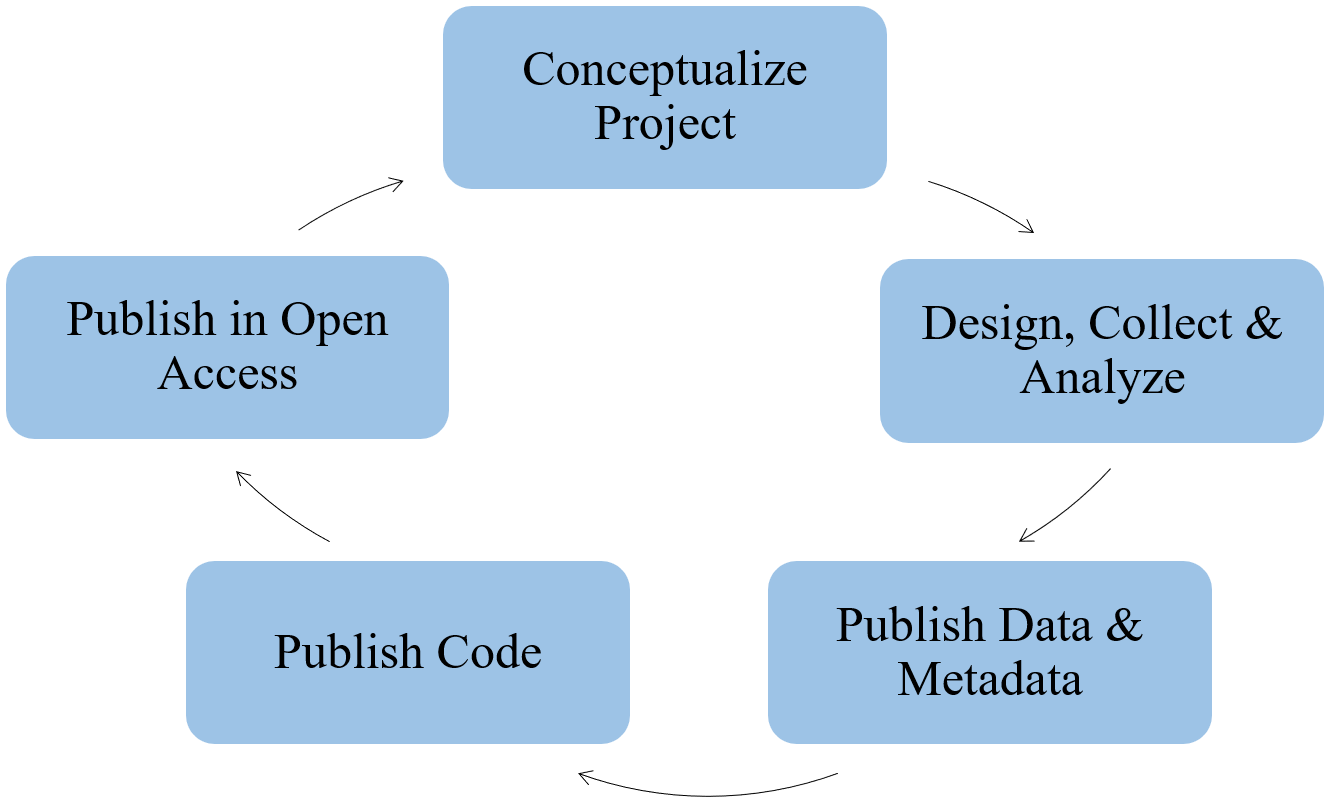
\includegraphics[width=\linewidth]{fig/scienceflow.png}
\end{minipage}
\hfill
\begin{minipage}{0.3\textwidth}
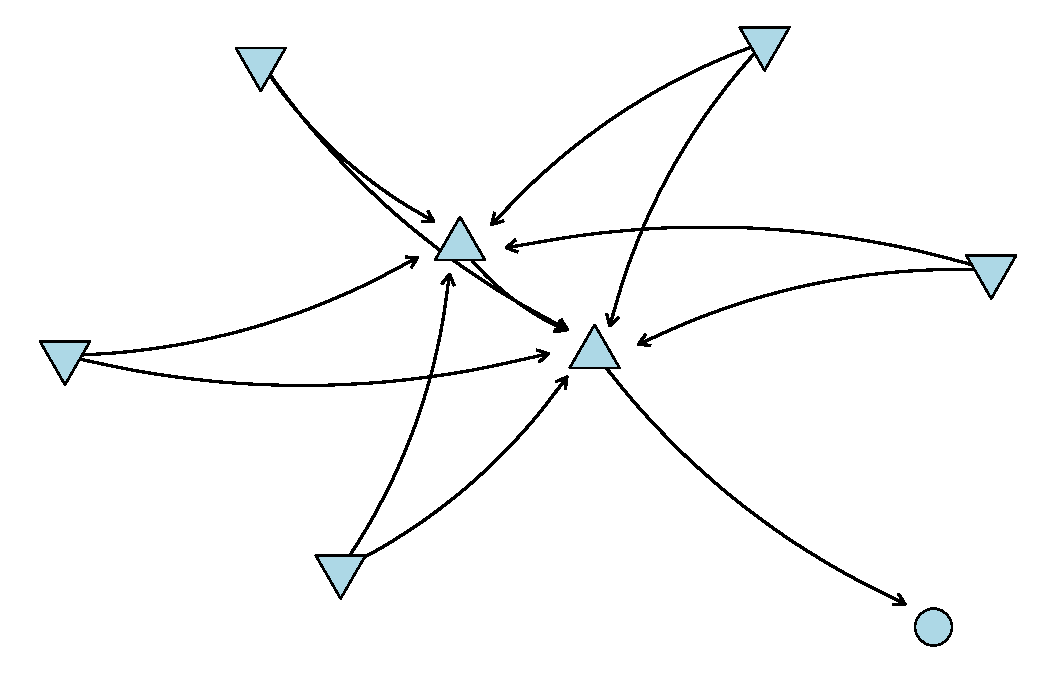
\includegraphics[width=\linewidth]{fig/titlefig.pdf}
\end{minipage}
}

%%%%%%
\begin{frame}[shrink]
\vspace{0.2in}
\titlepage
\end{frame}

\section{Background}

%%%%%%
\begin{frame}{{$\vcenter{\hbox{
\includegraphics[width=0.07\paperwidth]{fig/nceas_small.png}}}$\hspace{0.07in}\textbf{Open science workflow}}}
\centerline{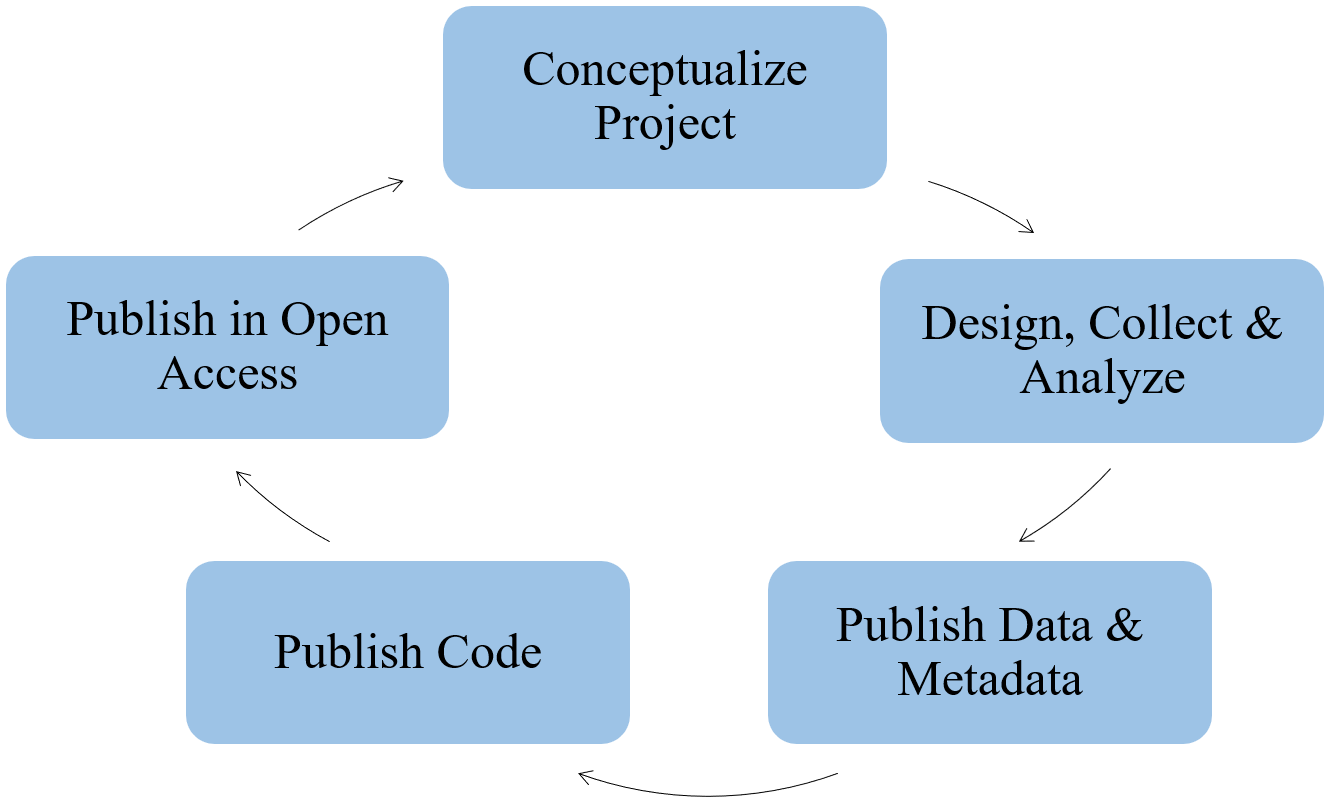
\includegraphics[width=0.85\textwidth]{fig/scienceflow.png}}
\vfill
\tiny
Modified from \href{https://esajournals.onlinelibrary.wiley.com/doi/full/10.1890/ES14-00402.1}{Hampton et al. 2015. The Tao of open science for ecology. Ecosphere 6(7):1-13.}
\end{frame}

%%%%%%
\begin{frame}[t]{{$\vcenter{\hbox{
\includegraphics[width=0.07\paperwidth]{fig/nceas_small.png}}}$\hspace{0.07in}\textbf{Open science workflow}}}

{\large \emtxt{Open Science for Synthesis: Gulf Research Program}}
\begin{columns}
\begin{column}{0.5\textwidth}
July 10 - July 28, 2017\\
NCEAS, Santa Barbara, CA 
\end{column}
\begin{column}{0.5\textwidth}
\hfill 
\includegraphics[width = \textwidth]{fig/nceas_full.png}
\end{column}
\end{columns}
\vspace{0.1in}
\begin{columns}
\begin{column}{0.5\textwidth}
\centerline{\fbox{\includegraphics[width = 0.85\textwidth]{fig/gom.jpg}}}
\end{column}
\begin{column}{0.5\textwidth}
\centerline{\fbox{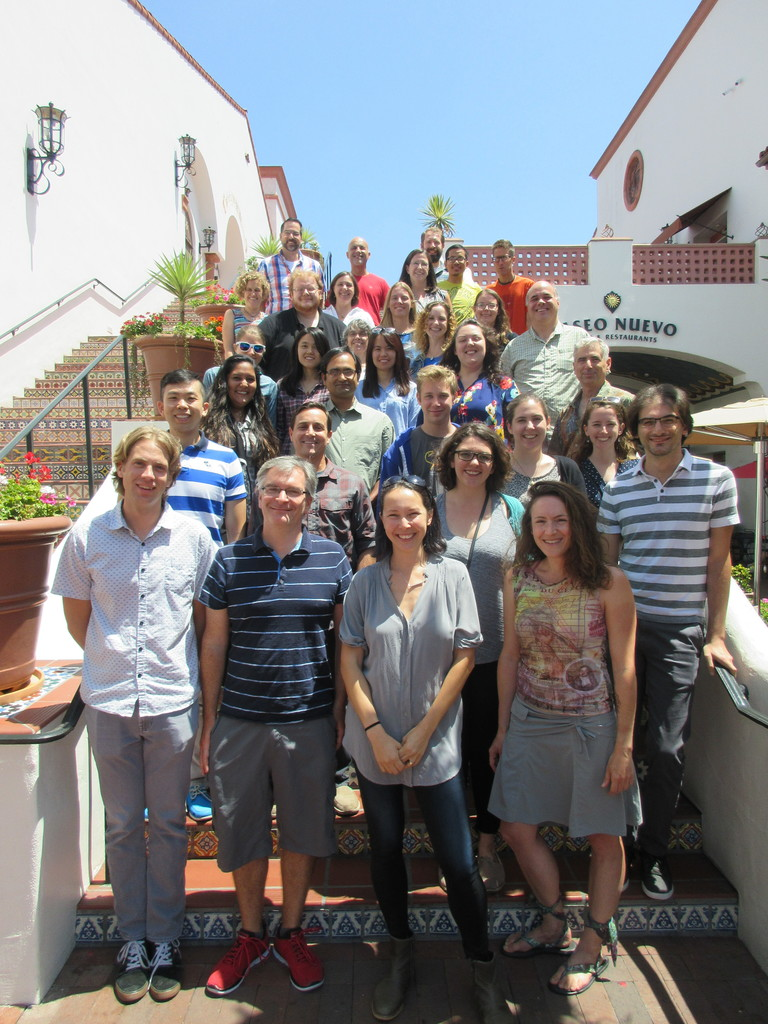
\includegraphics[width = 0.65\textwidth]{fig/ossgrp.jpg}}}
\end{column}
\end{columns}
\end{frame}

%%%%%%
\begin{frame}{{$\vcenter{\hbox{
\includegraphics[width=0.07\paperwidth]{fig/nceas_small.png}}}$\hspace{0.07in}\textbf{Today's talk}}}
\onslide<+->
Our experience using the open science workflow to inform restoration projects in estuaries \\~\\
\onslide<+->
Can we use disparate data to prioritize future restoration projects aimed at improving water quality? \\~\\
\begin{itemize}
\item<+-> \emtxt{Synthesize} data in space and time to evaluate cumulative effects of restoration projects\\~\\
\item<+-> \emtxt{Develop} a decision support tool with empirical observations to evaluate likelihood of potential outcomes \\~\\
\item<+-> \emtxt{Apply} the tool to guide expectations for future restoration projects
\end{itemize}
\end{frame}

%%%%%%
\begin{frame}{{$\vcenter{\hbox{
\includegraphics[width=0.07\paperwidth]{fig/nceas_small.png}}}$\hspace{0.07in}\textbf{Tampa Bay - from gross to less gross}}}
\begin{columns}
\begin{column}{0.5\textwidth}
\onslide<+->
\begin{center}
\fbox{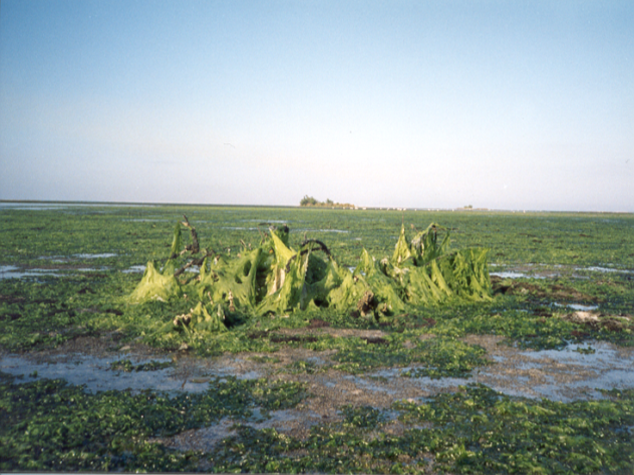
\includegraphics[width=0.7\textwidth]{fig/TB_Algae.png}}\\~\\
\fbox{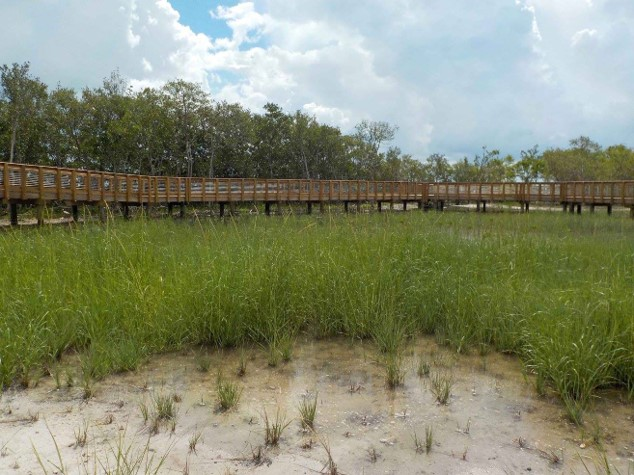
\includegraphics[width=0.7\textwidth]{fig/post_rest_sh.jpg}}\\~\\
\end{center}
\end{column}
\begin{column}{0.5\textwidth}
\emtxt{Past:}
\begin{itemize}
\item Mid-1970s N load 8.2$\times$10$^6$ yr$^{-1}$ {\footnotesize \cite{Greening06}}
\item Elevated chl-a concentrations
\item Increased occurrence of HABs
\end{itemize}
\onslide<+->
\emtxt{Present:}
\begin{itemize}
\item 2016 seagrass at \textasciitilde 17k ha {\footnotesize \cite{Sherwood17}}
\item Reductions in nutrient load, chlorophyll
\item Increase in water clarity {\footnotesize \cite{Morrison06,Beck17c}}
\end{itemize}
\end{column}
\end{columns}
\end{frame}

%%%%%%
\begin{frame}{{$\vcenter{\hbox{
\includegraphics[width=0.07\paperwidth]{fig/nceas_small.png}}}$\hspace{0.07in}\textbf{Tampa Bay - open data sources}}}
\begin{columns}
\begin{column}{0.5\textwidth}
\onslide<+->
\begin{center}
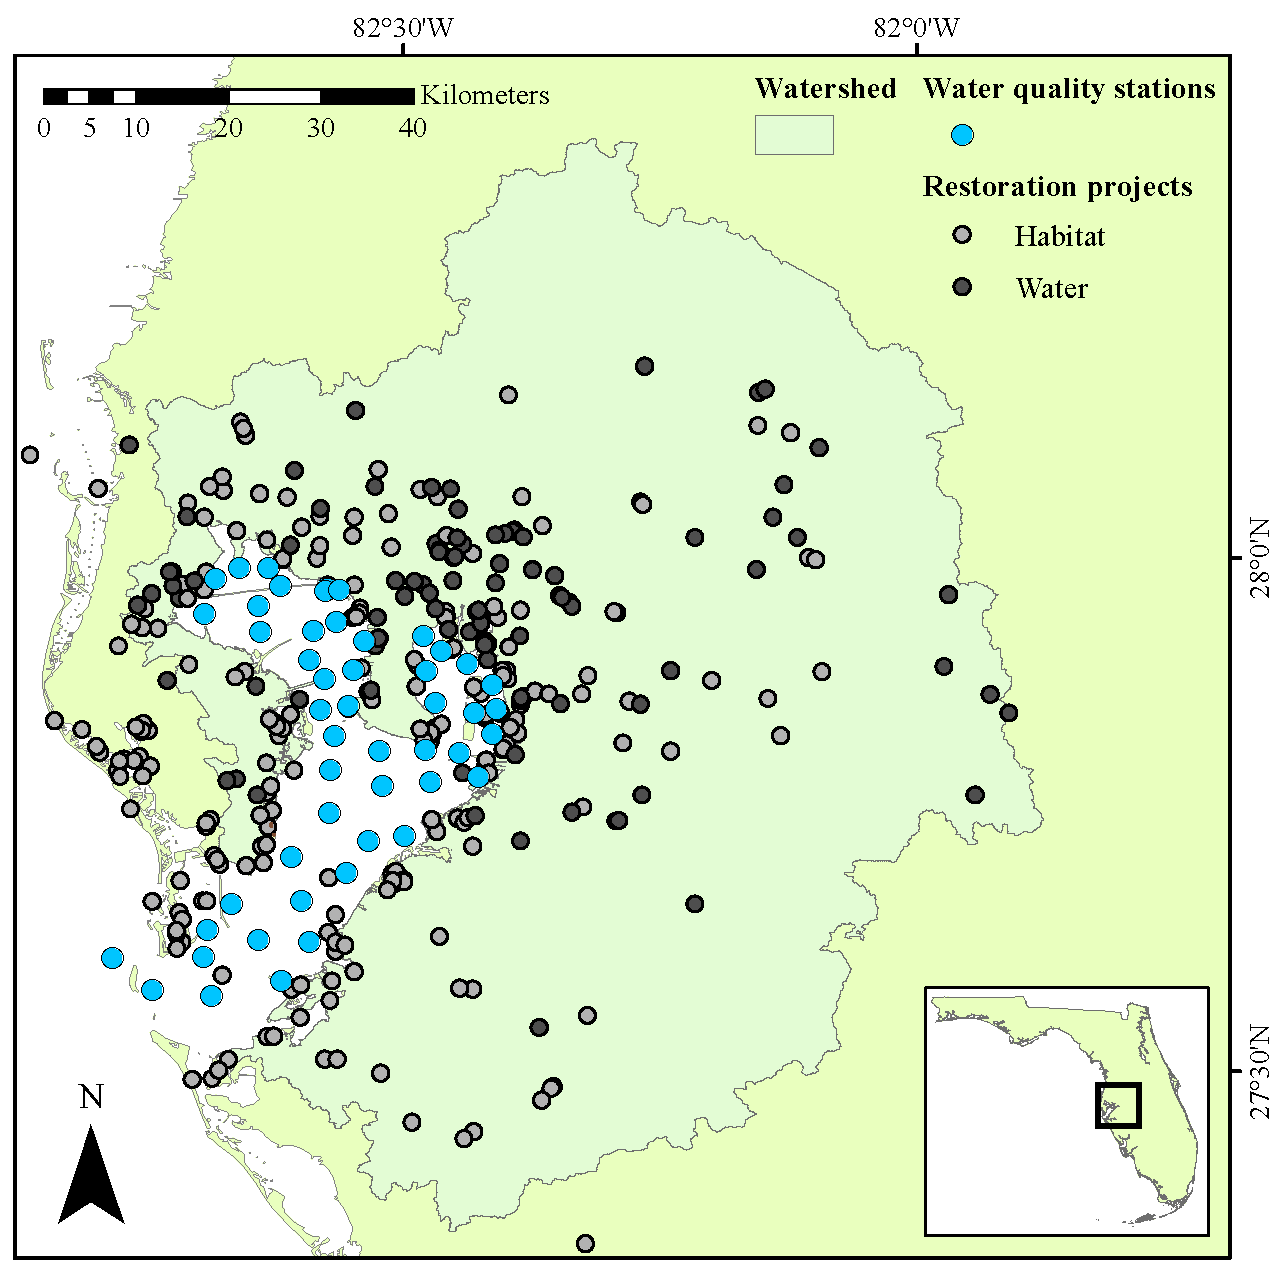
\includegraphics[width=0.95\textwidth]{fig/tbrest_map.pdf}
\end{center}
\end{column}
\begin{column}{0.5\textwidth}
\begin{itemize}
\item \emtxt{Water quality} monitoring dataset: 1974 to present, \textasciitilde 500 obs. per site \\~\\
\item<+-> \emtxt{Restoration projects} dataset: \textasciitilde 500 projects since 1971, habitat and water infrastructure projects
\end{itemize}
\end{column}
\end{columns}
\onslide<+->
\begin{center}
Despite considerable \emtxt{investments} in restoration, \emtxt{effectiveness evaluation} continues to elude practitioners at geographic scales {\footnotesize \cite{Diefenderfer16}}
\end{center}
\end{frame}

%%%%%%
\begin{frame}[t]{{$\vcenter{\hbox{
\includegraphics[width=0.07\paperwidth]{fig/nceas_small.png}}}$\hspace{0.07in}\textbf{Data munging with open source tools}}}
\emtxt{Task 1}: Can we empirically link 500 restoration projects to chlorophyll changes at water quality stations over a forty year period? 
\vfill
\centerline{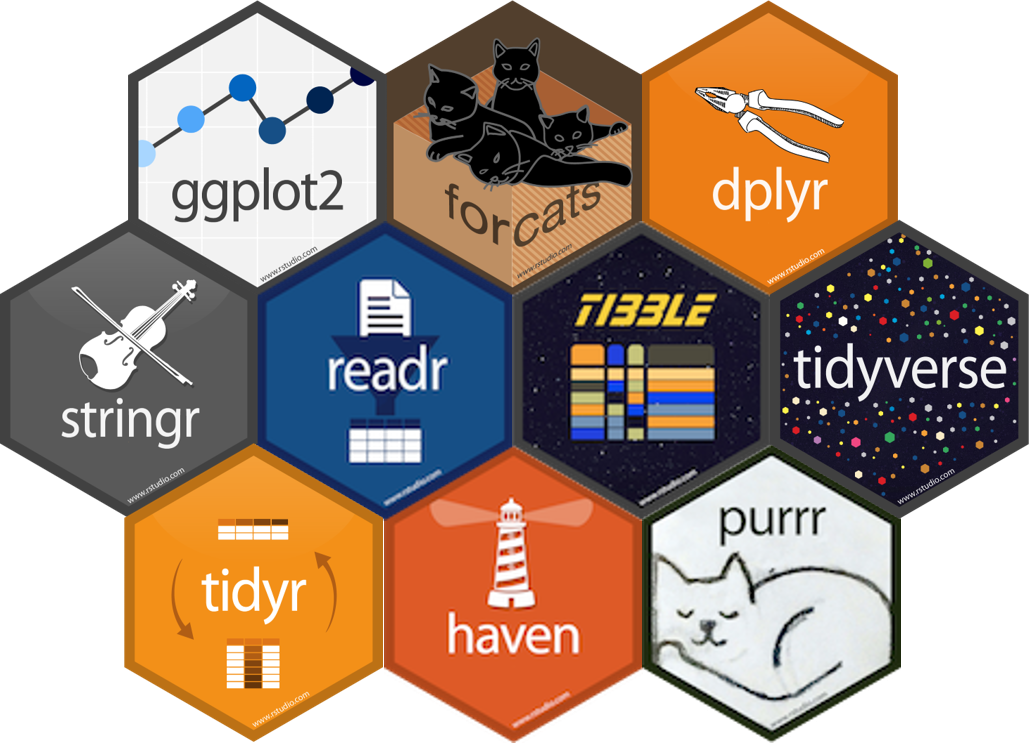
\includegraphics[width=0.65\textwidth]{fig/tidyverse.png}}
\end{frame}



%%%%%%
\begin{frame}{{$\vcenter{\hbox{
\includegraphics[width=0.07\paperwidth]{fig/nceas_small.png}}}$\hspace{0.07in}\textbf{Data munging with open source tools}}}
\onslide<1->
\begin{columns}
\begin{column}{0.5\textwidth}
\begin{overprint}
\begin{figure}
\centering
\includegraphics<1>[width=\textwidth]{fig/clomap1.pdf}
\includegraphics<2>[width=\textwidth]{fig/clomap2.pdf}
\includegraphics<3>[width=\textwidth]{fig/clomap3.pdf}
\includegraphics<4->[width=\textwidth]{fig/clomap5.pdf}
\end{figure}
\end{overprint}
\end{column}
\begin{column}{0.5\textwidth}
\onslide<1->
Can we link 500 restoration projects to chlorophyll changes over a forty year period? \\~\\
\begin{itemize}
\item<2-> Consider an effect of restoration \emtxt{site type}? \\~\\
\item<3-> Consider \emtxt{distance} of sites from water quality stations? \\~\\
\item<4-> Consider \emtxt{cumulative effects}? \\~\\
\end{itemize}
\end{column}
\end{columns}
\end{frame}



%%%%%%
\begin{frame}[t]{{$\vcenter{\hbox{
\includegraphics[width=0.07\paperwidth]{fig/nceas_small.png}}}$\hspace{0.07in}\textbf{Data munging with open source tools}}}
\onslide<1->
WQ and restoration sites: \emtxt{spatial join}
\begin{figure}
\centering
\includegraphics<1->[width=0.16\textwidth]{fig/ptplo.pdf}
\end{figure}
\begin{overprint}
\onslide<2>
WQ and restoration sites: \emtxt{temporal join}
\begin{figure}
\centering
\includegraphics<2>[width=\textwidth]{fig/tmplo1.pdf}
\end{figure}
\onslide<3>
WQ and restoration sites: \emtxt{temporal join, before/after}
\begin{figure}
\centering
\includegraphics<3>[width=\textwidth]{fig/tmplo2.pdf}
\end{figure}
\onslide<4>
WQ and restoration sites: \emtxt{temporal join, before/after, slice}
\begin{figure}
\centering
\includegraphics<4>[width=\textwidth]{fig/tmplo3.pdf}
\end{figure}
\end{overprint}
\end{frame}



%%%%%%
\begin{frame}{{$\vcenter{\hbox{
\includegraphics[width=0.07\paperwidth]{fig/nceas_small.png}}}$\hspace{0.07in}\textbf{Data munging with open source tools}}}
\onslide<1->
For \emtxt{many} water quality stations matched to \emtxt{many} restoration sites...\\~\\
\begin{overprint}
\begin{figure}
\centering
\includegraphics<1>[width = \textwidth]{fig/dens1.pdf}
\includegraphics<2->[width = \textwidth]{fig/dens2.pdf}
\end{figure}
\end{overprint}
\onslide<3>
\begin{tikzpicture}[overlay]
\draw[bend left=50,-latex,blue] (2.1, 6.07) to (6.85, 4.48);
\draw[bend left=60,-latex,red] (3.26, 5.7) to (7.7, 3.45);
\end{tikzpicture}
\end{frame}

%%%%%%
\begin{frame}{{$\vcenter{\hbox{
\includegraphics[width=0.07\paperwidth]{fig/nceas_small.png}}}$\hspace{0.07in}\textbf{Data munging with open source tools}}}
\onslide<1->
What is the probability of low/high chlorophyll given other events?\\~\\
\begin{center}
$P\left(Chl \mid Event\right) = \frac{P\left(Event \mid Chl\right) \cdot P\left(Chl \right)}{P \left(Event\right)}$ \\~\\
\end{center}
\onslide<2->
\begin{itemize}
\item Do water quality conditions differ by \emtxt{restoration type}?\\~\\
\item Does it differ by low/high \emtxt{salinity} as a natural covariate?\\~\\
\end{itemize}
\onslide<3->
\begin{center}
\emtxt{Bayesian models let us evaluate likelihood of potential outcomes given conditional distributions}
\end{center}
\end{frame}



%%%%%%
\begin{frame}{{$\vcenter{\hbox{
\includegraphics[width=0.07\paperwidth]{fig/nceas_small.png}}}$\hspace{0.07in}\textbf{Data munging with open source tools}}}
\onslide<1->
Using the \emtxt{conditional probabilities} from the \emtxt{empirical response}, what's the probability of low chlorophyll... 
\begin{columns}
\begin{column}{0.55\textwidth}
\onslide<1->
\begin{figure}
\centering
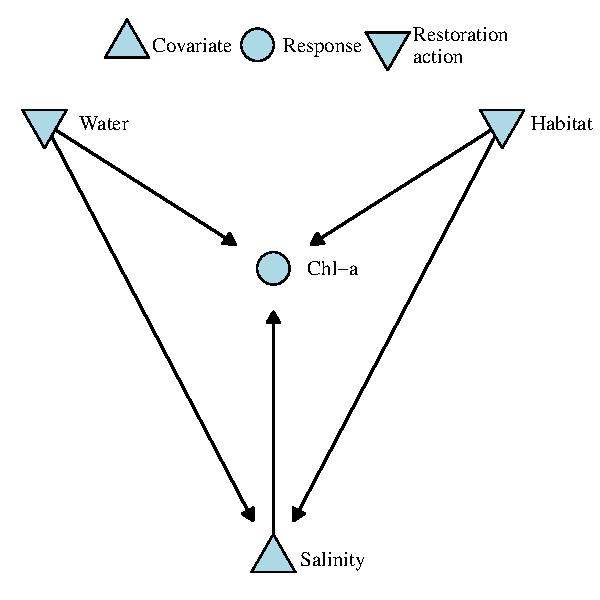
\includegraphics[width=\textwidth]{fig/simpnet.pdf}
\end{figure}
\end{column}
\begin{column}{0.45\textwidth}
\begin{itemize}
\item<2-> from water projects \\~\\
\item<3-> from habitat projects \\~\\ 
\item<4-> from all projects \\~\\
\item<5-> by salinity regime
\end{itemize}
\end{column}
\end{columns}
\end{frame}



%%%%%%
\begin{frame}{{$\vcenter{\hbox{
\includegraphics[width=0.07\paperwidth]{fig/nceas_small.png}}}$\hspace{0.07in}\textbf{Data munging with open source tools}}}
All possible scenarios:
\begin{figure}
\centering
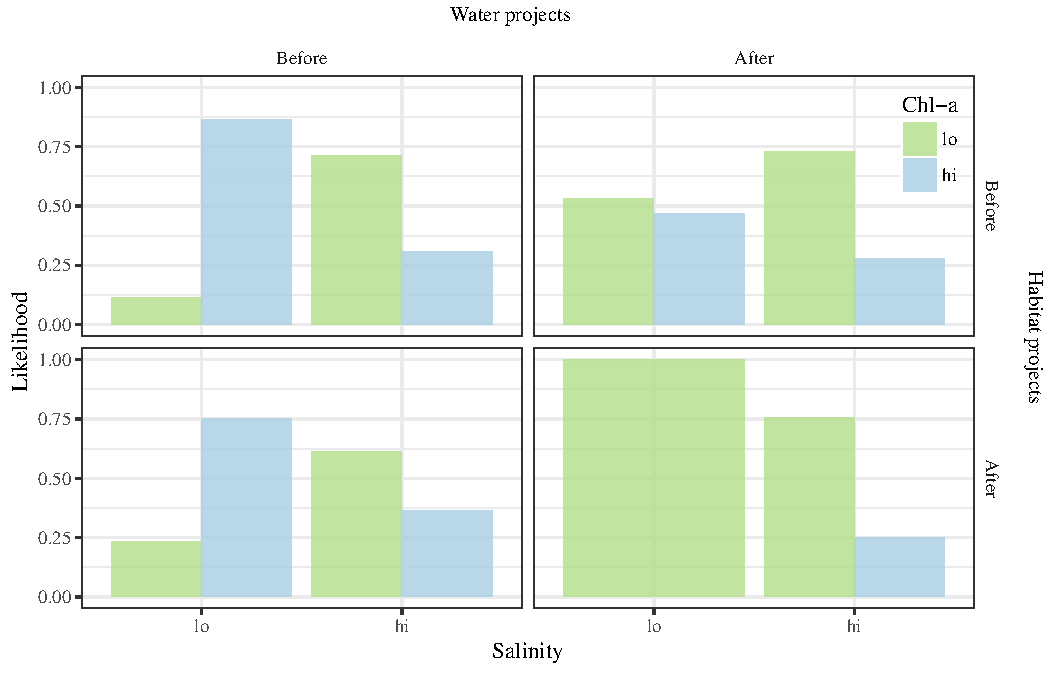
\includegraphics[width = 0.9\textwidth]{fig/chlpr1.pdf}
\end{figure}
\end{frame}



%%%%%%
\begin{frame}{{$\vcenter{\hbox{
\includegraphics[width=0.07\paperwidth]{fig/nceas_small.png}}}$\hspace{0.07in}\textbf{Data munging with open source tools}}}
\onslide<1->
\emtxt{Invidividual scenarios}: Probability of \textbf{high} chlorophyll\\~\\
\begin{columns}
\begin{column}{0.5\textwidth}
Water projects: \\~\\
\begin{itemize}
\item Before: 53\% \\~\\
\item After: 26\%
\end{itemize}
\end{column}
\begin{column}{0.5\textwidth}
Habitat projects: \\~\\
\begin{itemize}
\item Before: 50\% \\~\\
\item After: 50\%
\end{itemize}
\end{column}
\end{columns}
\onslide<2->
\vspace{0.2in}
\emtxt{Invidividual scenarios}: Probability of \textbf{low} chlorophyll\\~\\
\begin{columns}
\begin{column}{0.5\textwidth}
Water projects: \\~\\
\begin{itemize}
\item Before: 46\% \\~\\
\item After: 77\%
\end{itemize}
\end{column}
\begin{column}{0.5\textwidth}
Habitat projects: \\~\\
\begin{itemize}
\item Before: 49\% \\~\\
\item After: 51\%
\end{itemize}
\end{column}
\end{columns}
\end{frame}



%%%%%%
\begin{frame}{{$\vcenter{\hbox{
\includegraphics[width=0.07\paperwidth]{fig/nceas_small.png}}}$\hspace{0.07in}\textbf{Data munging with open source tools}}}
\onslide<1->
\emtxt{Where is the sweet spot}? \\~\\
Probability of low chlorophyll before/after \textbf{both project types} by \textbf{low/high salinity} \\~\\
\onslide<2->
\begin{columns}
\begin{column}{0.5\textwidth}
\emtxt{Low} salinity: \\~\\
\begin{itemize}
\item Before both projects: 13\% \\~\\
\item After both projects: 100\% \\~\\
\end{itemize}
\end{column}
\begin{column}{0.5\textwidth}
\emtxt{High} salinity: \\~\\
\begin{itemize}
\item Before both projects: 69\% \\~\\
\item After both projects: 75\% \\~\\
\end{itemize}
\end{column}
\end{columns}
\end{frame}

%%%%%%
\begin{frame}{{$\vcenter{\hbox{
\includegraphics[width=0.07\paperwidth]{fig/nceas_small.png}}}$\hspace{0.07in}\textbf{Data munging with open source tools}}}
\emtxt{Take home:} \\~\\
\begin{itemize}
\item<1-> Water infastructure projects had the largest effect
\item<2-> Habitat projects had an effect but less so
\item<3-> Effects most noticeable in low salinity zone
\end{itemize}
\vspace{0.2in}
\onslide<4-> \emtxt{But...} \\~\\
\begin{itemize}
\item<5-> Depends on year, distance combinations
\item<6-> This is a simple model
\end{itemize}
\end{frame}



%%%%%%
\begin{frame}{{$\vcenter{\hbox{
\includegraphics[width=0.07\paperwidth]{fig/nceas_small.png}}}$\hspace{0.07in}\textbf{Data munging with open source tools}}}
\emtxt{The holy grail:}
\begin{figure}
\centering
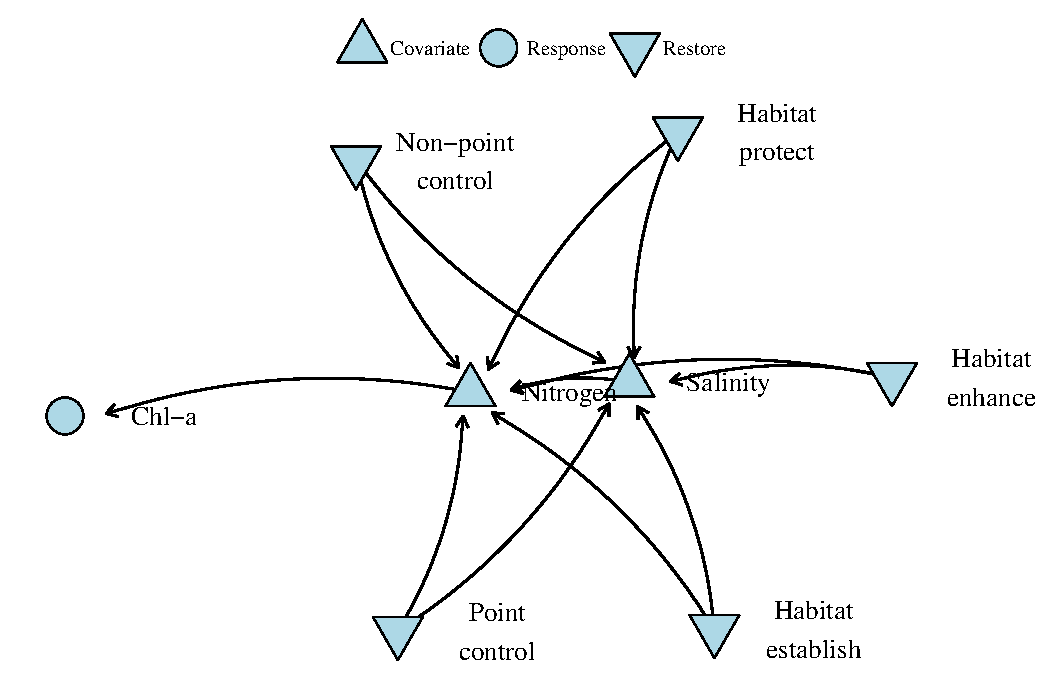
\includegraphics[width = 0.9\textwidth]{fig/compnet.pdf}
\end{figure}
\end{frame}

%%%%%%
\begin{frame}{{$\vcenter{\hbox{
\includegraphics[width=0.07\paperwidth]{fig/nceas_small.png}}}$\hspace{0.07in}\textbf{Open science workflow}}}
\centerline{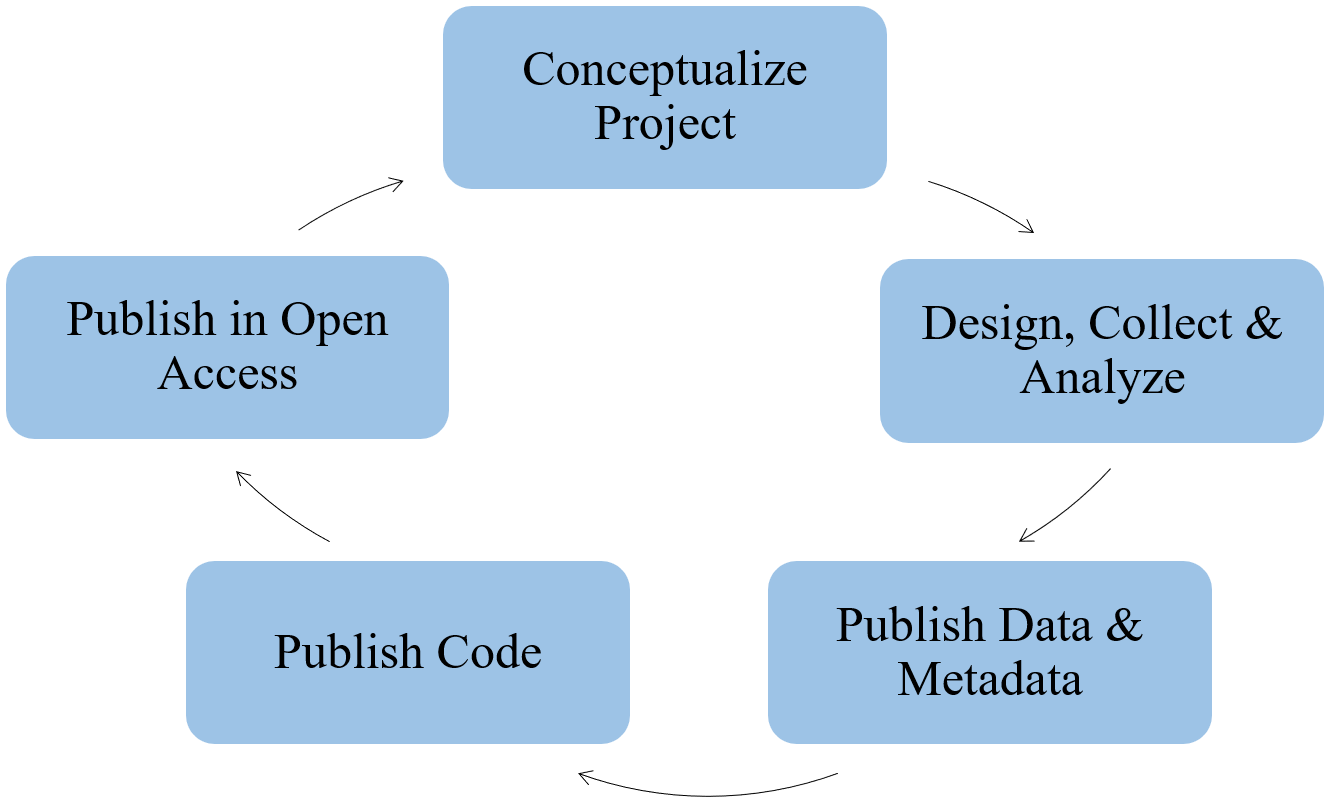
\includegraphics[width=0.85\textwidth]{fig/scienceflow.png}}
\vfill
\tiny
Modified from \cite{Hampton15}
\end{frame}

%%%%%%
\begin{frame}{{$\vcenter{\hbox{
\includegraphics[width=0.07\paperwidth]{fig/nceas_small.png}}}$\hspace{0.07in}\textbf{Open science workflow}}}
\onslide<1->
What aspects of our project used and benefitted from open science? \\~\\
\begin{itemize}
\item Early idea conception
\item Long distance collaboration
\item Transparent and reproducible analysis
\end{itemize}
\vspace{0.1in}
\begin{center}

\includegraphics[trim={0 0 3cm 0},clip,width = 0.9\textwidth]{fig/openfig.png}
\end{center}
\vspace{0.1in}
\onslide<2->
\centerline{\emtxt{... but the circle is not complete}}
\end{frame}

%%%%%%
\begin{frame}
\emtxt{Acknowledgments}:\\~\\
\begin{columns}
\begin{column}{0.8\textwidth}
{\footnotesize
Research staff and employees at NCEAS: M. B. Jones, A. Budden, T. Neal, B. Mecum, C. Lortie, L. Wasser, J. Brun  \\~\\
The Gulf Research Program \\~\\
Field staff and data managers at Hillsborough County Environmental Protection Commission}\\~\\
\end{column}
\begin{column}{0.2\textwidth}
\end{column}
\end{columns}
\vfill
\emtxt{Funding sources and contact}:\\~\\
\begin{columns}
\begin{column}{0.5\textwidth}
\centerline{
\includegraphics[width=\linewidth]{fig/nceas_full.png}}\\~\\
\vspace{0.15in}
\centerline{
\includegraphics[width=0.6\linewidth]{fig/grplogo.png}}
\end{column}
\begin{column}{0.5\textwidth}
\scriptsize
\href{mailto:marcusb@sccwrp.org}{marcusb@sccwrp.org}, 7147553217\\~\\

\includegraphics[width = 0.05\textwidth]{fig/git.png} GitHub (project): \href{https://github.com/fawda123/restorebayes}{https://github.com/fawda123/restorebayes}\\~\\

\includegraphics[width = 0.05\textwidth]{fig/git.png} GitHub (presentation): \href{https://github.com/fawda123/AWRA_2018}{https://github.com/fawda123/AWRA\_2018}\\~\\

\includegraphics[width = 0.05\textwidth]{fig/twitter.png} Twitter: @fawda123
\end{column}
\end{columns}
\vspace{0.2in}
\end{frame}


%%%%%%
\section{References}
\begin{frame}[t,shrink]{\textbf{References}}
\tiny
\setbeamertemplate{bibliography item}{}
\bibliographystyle{apalike_mine}
\bibliography{refs}
\end{frame}

\end{document}
